% \documentclass{article}
% %\usepackage[english]{babel}%
% \usepackage{graphicx}
% \usepackage{tabulary}
% \usepackage{tabularx}
% \usepackage[normalem]{ulem}
% \usepackage{cancel}
% \usepackage{tikz} 
% \usepackage{pdflscape}
% \usepackage{colortbl}
% \usepackage{lastpage}
% \usepackage{multirow}
% \usepackage{enumerate}
% \usepackage[shortlabels]{enumitem}
% \usepackage{color,soul}
% \usepackage{pdflscape}
% \usepackage{hyperref}
% %\usepackage[table]{xcolor}
% \usepackage{rotating}
% \usepackage{amsmath}
% \usepackage{fixltx2e}
% \usepackage{framed}
% \usepackage{mdframed}
% \usepackage[T1]{fontenc}
% \usepackage[utf8]{inputenc}
% \usepackage{textcomp}
% \usepackage{siunitx}
% \usepackage{ifthen}
% \usepackage{fancyhdr}
% \usepackage{gensymb}
% \usepackage{newunicodechar}
% \usepackage[document]{ragged2e}
% \usepackage[margin=1in,top=1.1in,headheight=57pt,headsep=0.1in]
% {geometry}
% \usepackage{ifthen}
% \usepackage{fancyhdr}
% \everymath{\displaystyle}
% \usepackage[document]{ragged2e}
% \usepackage{fancyhdr}
% \everymath{\displaystyle}
% \usepackage{empheq}

% \usepackage[most]{tcolorbox}

% \usepackage{booktabs} % Required for nicer horizontal rules in tables


% \usepackage{enumitem}

% %\usepackage[table,xcdraw]{xcolor}
% \usetikzlibrary{arrows}
% \linespread{2}%controls the spacing between lines. Bigger fractions means crowded lines%
% %\pagestyle{fancy}
% %\usepackage[margin=1 in, top=1in, includefoot]{geometry}
% %\everymath{\displaystyle}
% \linespread{1.3}%controls the spacing between lines. Bigger fractions means crowded lines%
% %\pagestyle{fancy}
% \pagestyle{fancy}
% \setlength{\headheight}{56.2pt}

% \definecolor{myblue}{rgb}{.8, .8, 1}
% \newcommand*\mybluebox[1]{%
% \colorbox{myblue}{\hspace{1em}#1\hspace{1em}}}

% \chead{\ifthenelse{\value{page}=1}{
\includegraphics[scale=0.3]{SCC}\\ \textbf \textbf Wastewater Constituents Analysis \& Laboratory Methods}}
% \rhead{\ifthenelse{\value{page}=1}{}{}}
% \lhead{\ifthenelse{\value{page}=1}{}{Wastewater Constituents Analysis \& Laboratory Methods}}
% \rfoot{\ifthenelse{\value{page}=1}{Module 1: WATR 048 - Spring 2019}{Module 1: WATR 048 - Spring 2019}}

% \lfoot{Shabbir Basrai}
% \cfoot{Page \thepage\ of \pageref{LastPage}}
% \renewcommand{\headrulewidth}{2pt}
% \renewcommand{\footrulewidth}{1pt}
% \begin{document}
% %\begin{empheq}[box=\mybluebox]{align}
% %a&=b\\
% %E&=mc^2 + \int_a^a x\, dx
% %\end{empheq}

% \newlist{steps}{enumerate}{1} % Defines "Steps" for enumerate as Step 1, Step 2 etc.
% \setlist[steps, 1]{label = Step \arabic*:} % Defines "Steps" for enumerate as Step 1, Step 2 etc.

% \setlist{nolistsep} % Reduce spacing between bullet points and numbered lists


%_______________________________________________________________________________________________________________________________________%
\chapterimage{Week6Digester.png} % Chapter heading image

\chapter{Digestion}


\section{Importance of Digestion}\index{Importance of Digestion}

		\begin{itemize}
		\item Solids (sludge) generated from the wastewater treatment processes contain organic compounds and also constituents that are beneficial plant nutrients. 
		\item However, the organic solids present in the sludge include pathogens and are also not stable (will putrefy)
		\item Thus, prior to the beneficial reuse of wastewater sludge or its disposal, sludge must be treated – stabilized to prevent odors and protect public health
		\item Additionally, if sludge is stabilized using anaerobic digestion, it  allows for the conversion of organic solids to yield valuable energy source - digester gas
		\end{itemize}
Sludge stabilization process results in the following:
		\begin{enumerate}
		\item Reduction in amount of solids - reducing biosolids hauling costs
		\item Pathogen reduction
		\item Odor reduction
		\item Reduction in vector attraction
		\item Product with beneficial reuse
		\end{enumerate}

Most common processes involved in sludge stabilization include:

		\begin{enumerate}
		\item Digestion - Aerobic or anaerobic
		\item Lime or alkaline stabilization
		\item Composting
		\item Long term storage in lagoons
		\item Thermal processes
		\item Incineration
		\end{enumerate}
		\begin{itemize}
		\item \hl{Sludge digestion is a microbiological process and is the most common sludge stabilization method}.
		\item There are two major sludge digestion processes:
			\begin{itemize}
			\item aerobic digestion which utilizes aerobic microorganisms, and produces carbon dioxide as a byproduct
			\item anaerobic digestion which utilizes anaerobic microorganisms and it produces digester gas as a byproduct.
			\item Digester gas is typically composed of 60-65\% methane gas with the remainder being mostly carbon dioxide ($CO_2$) and is useful because of its potential use as fuel - energy recovery from wastewater.
			\end{itemize}
		\end{itemize}

\section{Anaerobic Digestion Process Basics}\index{Anaerobic Digestion Process Basics}

		\begin{itemize}
		\item Solids removed from the primary and secondary treatment processes is fed to the digesters.  
		\item The sludge feed to the digesters range between 3 – 6\% total solids which typically contain 70\% organic solids
		\item The anaerobic digester is typically a large cylindrical concrete tank and is operated as a continuous process at a fixed volume\\ $\implies$ as sludge is fed into the digester it displaces an equal amount of sludge which leaves the digester.
\begin{center}
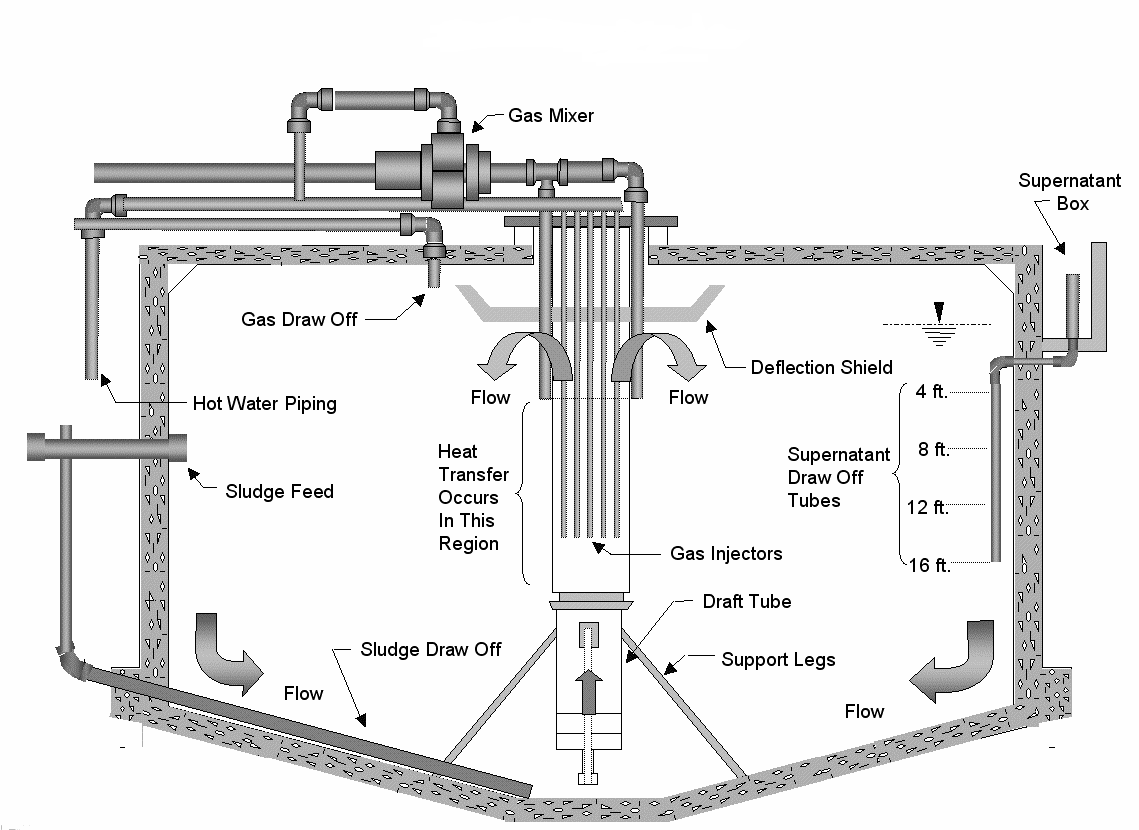
\includegraphics[scale=0.50]{DigesterFixedCover}\\
\textbf{Anaerobic Digester}\\
\end{center}
		\item The sludge typically occupies 70 - 90\% of the total digester volume and the methane carbon dioxide gas mixture occupies the headspace from where it is withdrawn also on a continuous basis.
		\item In the anaerobic digestion process microorganisms convert volatile matter into mainly methane (CH$_4$) and carbon dioxide (CO$_2$)
		\item The sludge content of the digesters is kept mixed and maintained in a constant temperature range using external heating.
		\item The activity and type of bacteria present in the digester is dictated by the operating temperature of the digester.
		\item Anaerobic digestion can be in the following three temperature ranges, each of which has its own unique microbiology.\\
			\begin{enumerate}[1. ]
			\item Psychrophilic digester:  Digester is maintained between 50  - 65 F.  Sludge detention time - 50 to 180 days
			\item Mesophilic digesters: – Digester is most commonly operated  between 95 – 98 F and the typical number of days required for digestion is between 15 to 30 days.\\
			\item Thermophilic digesters:  These digesters’ optimal operating temperatures range is between 113   135 F and it typically requires 5 to 12 days.\\
			\end{enumerate}     
		\item These organic solids are measured as volatile solids (VS).  
		\item The volatile solids content of the sludge entering and leaving the digester are measured to quantify the solids removal in the digester
		 \item Breakdown of volatile matter in the sludge ultimately into methane (CH$_4$) and carbon dioxide (CO$_2$) occurs in multiple steps involving different groups of microorganisms as follows:\\
			\begin{enumerate}[Step 1.]
			\item Hydrolysis:  Here the microorganisms breakdown complex organic matter in the sludge - carbohydrates, proteins, lignin, and lipids into simpler compounds including sugars, soluble fatty acids and amines.\\
			\item Acid Formation:  The simpler compounds formed in Step 1 are converted to organic acids by acid forming bacteria\\
			\item Methane Formation: The organic acids formed in Step 2 are converted into methane and carbon dioxide by methane forming bacteria.\\
			\end{enumerate}
		\item Gas production ranges between 10 to 16 cubic feet per pound of volatile matter destroyed and the gas production remains stable over time.
		\item Low gas production indicates problems - toxicity, temperature, volatile acid to alkalinity ratio, mixing, or feed rates.
		\end{itemize}
\section{Digester Calculations}\index{Digester Calculations}
\subsection{Sludge Pumping}\index{Sludge Pumping}
			
				\hl{Example Problems:}\\
					\begin{enumerate}
						\item A primary clarifier receives an average flow of 12 MGD containing 280mg/L of TSS.  This clarifier typically removes 75\% TSS  and produces a 3.5\% sludge and the sludge pump is rated to pump 35 cu.ft/min.
							\begin{enumerate}[a.]
								\item How many pounds of TSS is removed in the clarifier?

								\item How many cu.ft of sludge at the given 3.5\% sludge needs to be pumped per day to remove the solids?

								\item How many minutes would the sludge pump need to be operational each day to pump the required amount of sludge - calculated from ii.  above?

								\item For how many minutes each hour the sludge pump should be programmed to operate (Given the number of minutes the pump need to operate per day calculated from iii. above) ?\\
							\end{enumerate}
						Solution:\\
							\begin{enumerate}[a.]
								\item $lbs \enspace solids \enspace removed=(280*0.75)mg/l*12MGD*8.34=\boxed{21,017 \enspace lbs \enspace solids \enspace per \enspace day}$\\
								\vspace{0.5cm}
								\item $\dfrac{21,017 \enspace lbs \enspace solids}{day} = \dfrac{x \enspace \cancel{ft^3\enspace sludge}}{day} *\dfrac{7.48 \enspace \cancel{gal \enspace sludge}}{\cancel{ft^3 \enspace sludge}}* \dfrac{0.035 \enspace lbs \enspace solids}{1 \enspace \cancel{ {lb \enspace sludge}}}*\dfrac{8.34 \enspace \cancel{lb \enspace sludge}}{\cancel{gal \enspace sludge}}$\\
								\vspace{0.5cm}
								$\dfrac{x \enspace ft^3\enspace sludge}{day}= \dfrac{21,017}{0.035*834*7.48}=\boxed{9,626\dfrac{ft^3 \enspace sludge}{day}} $\\
								\vspace{0.5cm}
								\item $\dfrac{9,626 \enspace ft^3 \enspace sludge}{day}*\dfrac{min}{35 \enspace ft^3 \enspace sludge}=\boxed{\dfrac{275 \enspace minutes}{day}}$\\
								\vspace{0.5cm}
								\item $\dfrac{275 \enspace minutes}{day}*\dfrac{day}{24 \enspace hrs}=\boxed{\dfrac{11.4 \enspace minutes}{hr}}$\\
							\end{enumerate}
								\vspace{0.2cm}
						\item Calculate the lbs/day of solids removed in a primary clarifier treating a 5 MGD flow with an average influent and effluent TSS concentrations of 250 mg/l and 98 mg/l respectively.
						\vspace{0.2cm}
						Solution:\\
						\vspace{0.2cm}
						$\dfrac{lbs}{day}=5 MGD *(250-98)\dfrac{mg}{l}*8.34 = \boxed{6338\dfrac{lbs}{day}}$
				\end{enumerate}
\subsection{Digester VS or Organic Loading}\index{Digester VS or Organic Loading}				
				\hl{Example Problems:}\\

				\begin{enumerate}
					\item How many pounds of TS and VS are pumped to a digester each day if the digester receives 10,000 gpd of sludge at 5\% solids concentration with an average VS\% of 75\%?\\
					Solution:\\

					Digester TS loading (lbs/day)\\
					\vspace{0.3cm}
						$
							\dfrac{lbs \enspace TS}{day}
							=
							\dfrac{10,000 \enspace gal \enspace sludge}{day}
							*
							\dfrac{(8.34*0.05) lbs \enspace TS )}{gal \enspace sludge}
							=4,170
							\dfrac{lbs \enspace TS}{day}
						$
						\\
						\vspace{0.3cm}
						Digester VS loading (lbs/day)\\
						\vspace{0.3cm}
						$=4,170 	\dfrac{lbs \enspace TS}{day}*0.75\dfrac{lbs \enspace VS}{lb \enspace TS}=\boxed{3,128 \dfrac{lbs \enspace VS}{day}}$
						\vspace{0.5cm}
						\item An anaerobic digester is 37’ in diameter and 27’ deep with a 5,000 gallon daily sludge flow. The sludge is 6\% solids and 66\% volatile solids.  What is the volatile solids loading in pounds per cubic foot per day?
							
							
						Solution:\\
						{
						$
							Digester \enspace volatile \enspace solids 			\enspace loading \enspace rate = 					\dfrac
							{
							Digester \enspace Loading 
								\dfrac
								{
								lbs \enspace VS
								}
								{
								day
								}
							}
							{
							Digester \enspace volume (V)ft^3
							}
						$
						}\\
						\begin{center}
						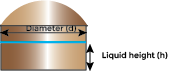
\includegraphics[scale=1]{DigesterWOCDimensions_1}
						\end{center}

						{
						$=\dfrac
							{
								5000
								\dfrac
									{gal \enspace sludge}
									{day}
								*(8.34*0.06*0.66) 
								\dfrac
									{lbs \enspace VS}
									{gal \enspace  sludge}
							}
							{
								(\dfrac
									{\pi}
									{4}*37^2*27)ft^3
							}
						=\boxed
							{
								0.057 \dfrac
									{lbs \enspace VS}
									{day-ft^3}
							}
						$}
				\end{enumerate}
\subsection{Total volatile solids (VS) reduction}\index{Total volatile solids (VS) reduction}	
				\begin{itemize}
					\item This provide a measure of the organic matter content removed and converted into digester gas in the digester. 
					\item Higher volatile solids reduction implies higher gas production and lower biosolids hauling costs.\\
					\item The VS reduction of the digester is provided by the Van Kleeck equation \\ 

					$$Digester \enspace VS \enspace reduction (\%)=\dfrac{VS_{in}-VS_{out}}{VS_{in}-VS_{in}*VS_{out}}*100$$

					\item Digester volatile solids concentration is typically expressed as a percentage of the sludge total solids.\\
					\item 70\% VS which means that 70\% of the total solids is volatile solids.
					\item \hl{The value of $VS_{in}$ and $VS_{out}$ for the digester VS reduction (Van Kleek) equation above should be in fraction and not as a percentage.}\\
					\vspace{0.2cm}
					A value of 0.7 should be used in the equation if the VS concentration is 70\%. Likewise, as 0.525 if the VS concentration is 52.5\%.\\
					\vspace{0.2cm}
					Applying this equation to calculate the digester VS reduction if the inlet sludge VS averages 75\% and the outlet sludge is 58\%?\\
					\vspace{0.3cm}
					\hl{Example Problem:}\\
					Calculate the \% VS reduction in a digester given the volatile solids content of the influent sludge to the digester is 70\% and the volatile solids content of the sludge leaving the digester is 52.5\%\\
					Solution:  $Digester \enspace VS \enspace reduction (\%)=\dfrac{0.7-0.525}{0.7-0.7*0.525}*100=\boxed{ 53\%}$\\
					\vspace{0.2cm}
				\end{itemize}

\chapterimage{Week6Chlorination.jpg} % Chapter heading image

\chapter{Chlorination}


\begin{itemize}
\item Treated wastewater effluent is disinfected prior to its discharge into a water body inorder to destroy pathogens primarily to prevent spread of waterborne disease and minimize public health problems
\item Chlorine is a very effective disinfectant and is the most widely used disinfectant for wastewater 
\item Chlorine disinfection is a practical and economical means for disinfecting large quantities of wastewaters which have been treated to various degrees. 
\item However, due to its toxicity, associated risk factors and its rising cost, use of ultraviolet light and ozone for wastewater disinfection is on the rise
\end{itemize}


\section{Forms of Chlorine}\index{Forms of Chlorine}

\begin{itemize}
	\item Due to safety issues related to the use of chlorine gas, 			\textbf{hypochlorites} are often used in lieu of chlorine
	\item Types of hypochlorites
	\begin{itemize}
	\item Sodium hypochlorite (NaOCl) comes in a liquid form which contains up to 12.5\% chlorine
	\item Calcium hypochlorite (Ca(OCl)$_2$), also known as HTH, is a solid which is mixed with water to form a hypochlorite solution. Calcium hypochlorite is 65-70\% concentrated.
	\end{itemize}
	\item Hypochlorites decompose in strength over time while in storage. Temperature, light, and physical energy can all break down hypochlorites before they are able to react with pathogens in water. 

\end{itemize} 

\section{Chlorine Properties}\index{Chlorine Properties}

\begin{itemize}
\item Chlorine is a yellowish-green gas at room temperature and atmosphric pressure
\item Chlorine gas can be pressurized and cooled to its liquid form for making it easy to ship and store. 
\item When liquid chlorine is released, it quickly turns into a gas that stays close to the ground (being heavier than air) and spreads rapidly.
	\item 	While it is not explosive or flammable, as a liquid or gas it can react violently with many substances 
	\item Chlorine is only slightly soluble in water (0.3 to 0.7\% by weight.) 
	\item Chlorine gas has a greenish-yellow color 
	\item It has a characteristic disagreeable and pungent odor, similar to chlorine-based laundry bleaches, and is detectable by smell at concentrations as low as 0.2 to 0.4 ppm
	\item It is about two and a half times as heavy as air
	\item One volume of liquid chlorine yields about 460 volumes of chlorine gas. 
	\item Liquid chlorine is amber in color and is about one and a half times as heavy as water 
	\item Chlorine is an irritant to the eyes, skin, mucous membranes, and the respiratory system 
\end{itemize}


\section{Chlorine Storage and Safety}\index{Chlorine Storage and Safety}


\subsection{Chlorine Delivery}\index{Chlorine Delivery}

\begin{itemize}
\item Typically for smaller plants chlorine gas is shipped in  pressurized steel cylinders - 150 lb or 2000 lb (ton cylinder) size
\item Larger plants may get their chlorine supply in rail tank cars
\item The daily chlorine usage is typically established based upon the weighing of the chlorine containers.
\end{itemize}


\subsection{Chlorine Leak Response}\index{Chlorine Leak Response}
\begin{itemize}
	\item Typically for smaller plants chlorine gas is shipped in  pressurized steel cylinders - 150 lb or 2000 lb (ton cylinder) size.  Larger plants may get their chlorine supply in rail tank cars.  
	\item The daily chlorine usage is typically established based upon the weighing of the chlorine containers.
	\item The withdrawal rates from a chlorine cylinder is based on the temperature of the liquid in the cylinder, and thus the pressure of the gas. 
	\item As chlorine gas is withdrawn from the cylinder, it absorbs the heat from the surroundings.
	\item For low withdrawal rates, heat will be able to be transferred from the surrounding air to the container in time so that there is no drop in temperature or pressure, 
	\item If the chlorine withdrawal is larger, the air will not be able to transfer the heat quickly enough and the temperature (and pressure) of the chlorine will drop, thus resulting in a lower feed rate. 
	\item If high enough and prolonged enough, this can even result in ice formation around the outside of the container, further decreasing the withdrawal rate. 
	\item The most effective way to increase withdrawal rate from a single container is to circulate the surrounding air with a fan. Again, never apply heat to the containers.
	\item If chlorine gas escapes from a container or system, being heavier than air, it will seek the lowest level in the building or area
	\item Only trained staff with access to proper personal protection equipment (PPE) including self-contained breathing apparatus, should handle the chlorine cylinders and address chlorine leak issues 
	\item When a leak is suspected, it is recommended that ammonia vapors be used to find the source. When ammonia vapor using a rag or brush, is directed at a leak, a white cloud will form. To produce ammonia vapor, a plastic squeeze bottle containing about 5 \% ammonia, aqua ammonia (ammonium hydroxide solution) should be used. A weaker solution such as household ammonia may not be concentrated enough to detect minor leaks
	\item All safety equipment should be located outside of the chlorine room and be easily accessed by all personnel
	\item Small leaks around valve stems can usually be corrected by tightening the packing nut or closing the valve. A leak can also be reduced by removing the chlorine as rapidly as possible
	\item If it cannot be added to the process there are several chemicals which can be used to absorb the chlorine gas. For example, chlorine can be absorbed by using 1$frac{1}{4}$ pounds of caustic soda or hydrated line, or 3 pounds of soda ash per pound of chlorine. 
	\item If the leaking container can be moved, it should be transported to an outdoors area where minimal harm will occur. Keep the leaking part the most elevated so that gaseous chlorine will leak rather than liquid chlorine.
	\item If the leak is large, all persons in the adjacent area must be warned and evacuated. Only authorized persons equipped with the proper breathing apparatus, and protective measures to the eyes and body should investigate. 
	\item As water is not an efficient absorbent for chlorine and the fact that chlorine reacts with water to form very corrosive hydrochloric acid, never apply water to a leak or consider submerging a chlorine cylinder (for example, in a pond or tank), since it will probably float.
	\item Remember to keep windward of the leak.
	\item As chlorine cylinders pressure increases with temperature, as a safety measure the chlorine cylinders are fitted with fusible plug which melts between 158$^o$ and 165$^o$ F.
	\item Keep chlorine cylinder or container emergency repair kits available. Be familiar with their use and location.
	\item Leaks at fusible plugs and cylinder valves requires special handling and emergency equipment. The chlorine supplier must be notified immediately
	\item Pin hole leaks in cylinder walls or ton tanks can usually be stopped by mechanical pressure applications (clamps, turnbuckles, etc.). This only temporary and may require your ingenuity.
	\item Leaking containers cannot be shipped.
	\item In general, daily inspection of all chlorine cylinders will avoid major problems
\end{itemize}

\subsection{Chlorine Reactions Related to Disinfection}\index{Chlorine Reactions Related to Disinfection}
\textbf{Chlorine reacts with water to form hypochlorous and hydrochloric acids}\\
Cl$_2$ \hspace{0.8cm}	+ \hspace{0.3 cm}	 H$_2$O		\hspace{0.8cm} $\iff$ 
\hspace{0.8cm} HOCl	\hspace{0.8cm}	 +	\hspace{0.8cm}	 HCl \\
chlorine \hspace{0.8cm}	water \hspace{1.8cm}		 hypochlorous acid	\hspace{0.1cm}	 hydrochloric acid\\ 
	\vspace{0.5cm}
	\begin{itemize}
		\item Hypochlorous acid dissociates in water to form the hydrogen and hypochlorite ions\\
 HOCl \hspace{1.8 cm} $\iff$ \hspace{1.8 cm} H$^+$ \hspace{1.8cm} + 	\hspace{0.8cm}OCl$^-$\\ 
hypochlorous acid  \hspace{1.9 cm}      hydrogen ion   \hspace{1.5cm}           hypochlorite ion

		\begin{itemize}
			\item Hypochlorous acid is the most effective form of chlorine available to kill microorganisms
			\item Hypochlorite ions is much less efficient disinfectant
		\end{itemize}

		\item The concentration of hypochlorous acid and hypochlorite ions in chlorinated water will depend on the water's pH
		\begin{itemize}
			\item A higher pH facilitates the formation of more hypochlorite ions and results in less hypochlorous acid in the water
		\end{itemize}
		\item A significant percentage of the chlorine is still in the form of hypochlorous acid even between pH 8 and pH 9
		\end{itemize}



\section{Chlorine Disinfection}\index{Chlorine Disinfection}

\begin{itemize}
\item When chlorine is added to a wastewater flow, it will first react or combine with certain organic and inorganic substances present, prior to acting on pathogens.  The amount of chlorine used up as part of these reactions is referred to as the \textbf{chlorine demand}\\

\item The \textbf{free chlorine} remaining after the chlorine demand is satisfied, is the strongest form of chlorine available for disinfection.  

\item Chlorine combined with ammonia (as chloramines) and organic compounds (as chloroorganic compounds), known as \textbf{combined chlorine} also exhibit disinfecting properties - albeit weaker than the free chlorine.

\item \text{Total residual chlorine} is the sum of free chlorine and combined chlorine and it is the residual chlorine concentration which represents the amount of chlorine available for disinfection 

\item \textbf{Chlorine Demand = Applied Chlorine Dose - Chlorine Residual}\\ Chlorine residual should be the basis of measuring the effectiveness of chlorine disinfection

\item Chlorine residuals are measured in the field using a colorimeteric method.  In the laboratory, chlorine residuals are measured typically using: 1) Amperometric Titration, or 2) Iodometric Titration

\item Chlorine dosage is typically established from either bench scale laboratory testing, or actual measurement of field results. 

\item Since field conditions, particularly the mixing element, are not as well controlled as laboratory tests, the actual dosage is expected to be generally higher than from that established in the laboratory. 

\item Even though residual chlorine concentration can be used for establishing the effectiveness of disinfection, the ultimate effectiveness of disinfection can be monitored by conducting bacteriological testing.

\end{itemize}

\section{Factors Affecting Chlorine Disinfection Efficiency}\index{Factors Affecting Chlorine Disinfection Efficiency}

The disinfection efficiency of chlorine depends on the following factors:\\
\begin{itemize}
	\item pH:  Disinfection is more efficient at a low pH when large quantities of hypochlorous acid are present than at a high pH when hypochlorite ions is the dominant species in the water
	\item Concentration:  Contact Time Ratio (CT):  For effective chlorine disinfection both sufficient chlorine dosages – concentration (C) as well as contact time (T) are necessary.  There may be a substantial residual but if CT factor is not adequate, disinfection may not be effective. Generally both of these factors must be worked out experimentally for a given system
	\item Temperature:  Colder temperatures are less favorable for disinfection. 
Proper contacting or mixing or agitation:  This is necessary to make sure that the chlorine applied contacts or reaches the microbial cells
	\item Organic and inorganic material present:  The chlorine used by these organic and inorganic reducing substances including metal ions, organic matter and ammonia, is defined as the chlorine demand.  So that the amount of chlorine that has to be added to wastewater for different purposes will also vary.
\item Even though residual chlorine concentration can be used for establishing the effectiveness of disinfection, the ultimate effectiveness of disinfection can be monitored by conducting bacteriological testing.
\end{itemize}
		
\section{Dechlorination}\index{Dechlorination}
\begin{itemize}
\item Dechlorination is the process of removing residual chlorine from disinfected wastewater prior to discharge into the environment
\item Dehlorination is necessary to mitigate the toxic effect of chlorine on the receiving waters.  
\item Sulfur dioxide is most commonly used for dechlorination.
\item Other chemicals used for sodium bisulfite, sodium sulfite and sodium thiosulfate.
\end{itemize}

\section{Math Problems}\index{Math Problems}

\subsection{Establishing Chlorine Dosage}\index{Establishing Chlorine Dosage}

\hl{Example Problems:}
\begin{enumerate}
\item Calculate how many pounds per day of chlorine should be used to maintain a dosage of 12 mg/l at a 5.0 MGD flow.\\
Solution:\\
$lbs/day=conc. (mg/l)*flow(MGD)*8.34$\\
$lbs/day=12*5*8.34=\boxed{500.4lbs/day}$\\

\subsection{Calculating Dosage/Residual/Demand Concentrations}\index{Calculating Dosage/Residual/Demand Concentrations}

\hl{Example Problems:}
\item If 80 pounds of chlorine are applied each day to a flow of 1.5 MGD, what is the dosage in mg/l?\\
Solution:\\
Applying the pounds formula:\\  $lbs/day=conc. (mg/l)*flow(MGD)*8.34$\\
$\implies conc. (mg/l)=\dfrac{lbs/day}{flow(MGD)*8.34}=\dfrac{80}{1.5*8.34}=\boxed{6.4mg/l}$

\item How many pounds per day of chlorine will be required to disinfect a secondary effluent flow of 1.68 MGD if the chlorine demand is found to be 8.5 mg/l and a residual of 3 mg/l is desired?
Chlorine dosage = chlorine demand + chlorine residual\\
$chlorine \enspace dosage=8.5+3=11.5mg/l$\\
$lbs/day=conc. (mg/l)*flow(MGD)*8.34=1.68*11.5*8.34=\boxed{161.2lbs/day}$\\
\end{enumerate}

\chapterimage{Week7Safety.png} % Chapter heading image

\chapter{Safety}
\section{Wastewater Treatment Hazards}\index{Wastewater Treatment Hazards}
There are many hazards encountered in wastewater treatment operations.  The hazards and their respective mitigation measures are as follows:\\
\subsection{Hazardous Chemicals}\index{Hazardous Chemicals}
\begin{itemize}
\item Hazardous chemicals are used throughout wastewater treatment plants and in collection systems. 
\item To understand the dangers of these chemicals and to take adequate steps OSHA requires that the chemical manufacturer, distributor, or importer provide Safety Data Sheets (SDSs) (formerly MSDSs or Material Safety Data Sheets) for each hazardous chemical to downstream users to communicate information on hazards related to that particular chemical or product.
\item Employers must ensure that the SDSs are available and readily accessible to employees for all hazardous chemicals in their workplace.
\item The SDS includes information such as the properties of each chemical; the physical, health, and environmental health hazards; protective measures; and safety precautions for handling, storing, and transporting the chemical.\\
\end{itemize}
\subsection{Hazardous Gasses}\index{Hazardous Gasses}
\begin{itemize}
\item A summary of the properties and effects of hazardous gases found in wastewater operations is provided in the table below.
\item To safeguard against the potential impacts of these gases, employees are required to follow practices including donning appropriate Personal Protective Equipment (PPE) and utilizing respiratory protection\\
\end{itemize}
\begin{center}
\includegraphics[scale=0.6]{SafetyHazardousGases4}\\ 
\end{center}

\subsection{Falls}\index{Falls}
\begin{itemize}
\item Falls are one of the leading causes of injuries and deaths on the job.  Fall protection is a combination of methods and devices used to protect workers from falling off, onto, or through working levels. 
\item Fall protection methods and devices are typically divided into two categories: those that prevent falls and those that arrest falls. 
\item Examples of fall protection methods and devices include rails, guards, guardrails, barriers, fall-arrest systems, safety nets, hole covers, and various work practices and procedures.
\end{itemize}
\begin{center}
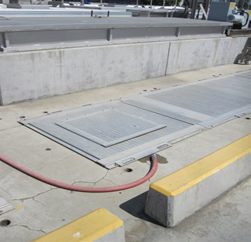
\includegraphics[scale=0.8]{SafetyFallProtection1}\hspace{1cm} 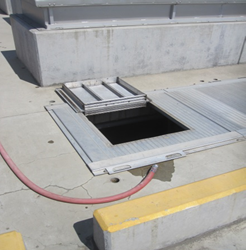
\includegraphics[scale=0.8]{SafetyFallProtection2}\\
\end{center}
\section{Noise}\index{Noise}
\begin{itemize}
\item Noise as a hazard is sound that is especially loud or impacting. 
\item A wastewater treatment plant has equipment that produces high noise levels both continuously and intermittently. 
\item As such, it is important to be aware of this hazard and to take preventive steps to reduce exposure to damaging noise levels by wearing effective hearing protection and to minimize the duration of the exposure to the noise.
\end{itemize}

\subsection{Electrical Hazards}\index{Electrical Hazards}
\begin{itemize}
\item Ordinary 120-V electricity can be fatal; most wastewater facility electrical systems operate at 120 to 4000 V or more.  
\item All voltages should be considered dangerous and potentially life threatening.  
\item Safe working rules and practices that should be followed when working on electrical systems
\item Before working on an electrical system, perform a job hazard analysis to determine any potential hazards and methods of abating those hazards
\end{itemize}


\subsection{Rotating and Moving Equipment}\index{Rotating and Moving Equipment}

\begin{itemize}
\item All rotating and moving equipment should be guarded. 
\item The best method for preventing machinery-related injuries is through use of equipment guards enforced through engineering and administrative controls.   
\item The best way to prevent this type of injury is to install point-of-operation guards that prevent contact with ingoing nip points, pinch points, rotating parts, flying chips, and sparks.
\end{itemize}
\begin{center}
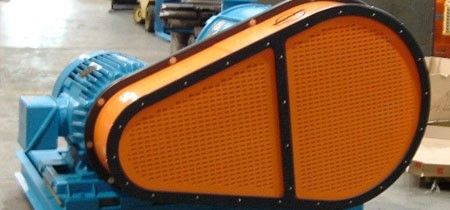
\includegraphics[scale=0.6]{SafetyMachineGuarding}\\
\end{center}

\subsection{Heat Stress}\index{Heat Stress}
\begin{itemize}
\item Heat stress falls into two categories: heat illness and heat stroke. 
\item Both are serious conditions and should not be taken lightly. 
\item Heat stress can result from: 
\begin{itemize}
\item High temperature and humidity, dehydration from low fluid consumption
\item Direct sun exposure (with no shade) or extreme heat, 
\item Limited air movement (no breeze or wind), 
\item Physical exertion, Use of bulky protective clothing and equipment, 
\item Poor physical condition or ongoing health problems, 
\item Some medications
\item Pregnancy
\end{itemize}
\end{itemize} 


\section{Safety Practices}\index{Safety Practices}
\subsection{Lockout - Tagout (LOTO)}\index{Lockout - Tagout (LOTO)}

When conducting routine inspections, repairs and maintenance activities, requires meeting the mandates of \hl{Occupational Safety  Hazard Administration(OSHAs) Lock-Out/Tag-Out (LOTO) program}\\
which is designed to prevent injury or fatalities.  It involves preventing an equipment from accidentally starting up and release of all stored energy.  Hazardous energy sources include: 
\begin{itemize}
\item Electrical 
\item Mechanical
\item Hydraulic
\item Pneumatic 
\item Chemical 
\item Thermal  
\item Other energy
\end{itemize}

The LOTO involves established and documented procedures specific to an equipment or machinery.  It typically comprises of:\\
\begin{itemize}
\item Notifying affected employees
\item Stopping and isolating the equipment
\item Releasing stored energy
\item Verification of the isolation and de-energization
\item Placing lock-out devices which use a positive means such as a lock, either key or combination type, to hold an energy isolating device in the safe position and prevent the energizing of a machine or equipment
\item Appropriately tagging the devices to indicate its non-operation and that it may not be operated until the tagout device is removed
\end{itemize}

\subsection{Personal Protective Equipment (PPE)}\index{Personal Protective Equipment (PPE)}
Employees depend on personal protective equipment to protect themselves from hazards and perform daily duties. PPE includes but is not limited to safety glasses, face shields, hard hats, gloves, foot protection, and durable and disposable chemical-protective clothing. Respirators and fall protection might also be required. However, respirators and fall protection fall under separate OSHA standards. \\

\subsection{Confined Space Entry}\index{Confined Space Entry}
OSHA defines a confined space as an area that:
\begin{itemize} 
\item is large enough and so configured that an employee's body can enter and perform assigned work
\item has limited or restricted means for entry or exit; and
\item is not designed for continuous employee occupancy.
\end{itemize}
A permit-required confined space is defined as a confined space that:
\begin{itemize} 
\item contains or has a potential to contain a hazardous atmosphere
\item contains a material that potentially could engulf an entrant
\item has an internal configuration that could trap or asphyxiate an entrant through inwardly converging walls or a floor that slopes downward and tapers to a smaller cross-section
\item contains any serious safety or health hazard
\end{itemize}

Potentially dangerous atmospheric conditions which can exist in confined spaces include: 
\begin{itemize}
\item Oxygen level: Some gasses are heavier than air and so will fill up a confined space, which forces oxygen out.  The oxygen concentration must not fall below 19.5\% at any time.  In plants where pure oxygen is used there is a potential hazard due to high the oxygen concentration.  Oxygen concentration greater than 23\% increases the risk of ignition and fire
\item Explosive conditions:  Many gasses are explosive when present in certain ratios with oxygen. These ratios are defined by the upper explosive limit(UEL) and the lower explosive limit (LEL).  The minimum concentration of a particular combustible gas or vapor necessary to support its combustion in air is defined as the Lower Explosive Limit (LEL) for that gas. Below this level, the mixture is too “lean” to burn. The maximum concentration of a gas
or vapor that will burn in air is defined as the Upper Explosive Limit (UEL). Above this level, the mixture is too “rich” to burn.  The range between the LEL and UEL is known as the flammable range for that gas or vapor.  
\item Toxic conditions:  This condition could potentially exist due to the presence of gasses such as carbon dioxide, chlorine and hydrogen sulfide.  
\end{itemize}



\includepdf[pages=-]{oshasds.pdf}
\includepdf[pages=-]{anhydammoniasds.pdf}
\end{document}